% This document is part of the EPRVCalibration project
% Copyright 2019 the authors. All rights reserved.

% style notes
% -----------
% - use \acronym and use \eprv, \lfc, and so on.

\documentclass[twocolumn]{aastex63}
\usepackage{xcolor}
\newcommand{\lz}[1]{\textcolor{orange}{#1}}

\usepackage[ruled,vlined]{algorithm2e}
\usepackage{graphicx}

% typesetting words
\newcommand{\project}[1]{\textsl{#1}}
\newcommand{\name}{\project{Excalibur}}
\newcommand{\acronym}[1]{{\small{#1}}}
\newcommand{\expres}{\project{\acronym{EXPRES}}}
\newcommand{\eprv}{\acronym{EPRV}}
\newcommand{\lfc}{\acronym{LFC}}

% math shih
\newcommand{\mps}{\mathrm{m\,s^{-1}}}

% margins and page setup, etc
\addtolength{\textheight}{1.00in}
\addtolength{\topmargin}{-0.50in}
\sloppy\sloppypar\raggedbottom\frenchspacing

\begin{document}
\title{\name:
A non-parametric, hierarchical model for a precision spectrograph}

\correspondingauthor{Lily Zhao}
\email{lily.zhao@yale.edu}

\author[0000-0002-3852-3590]{Lily Zhao}
\affil{Yale University, 52 Hillhouse, New Haven, CT 06511, USA}

\author[0000-0003-2866-9403]{David W. Hogg}
\affil{Center for Cosmology and Particle Physics, Department of Physics, New York University, 726 Broadway, New York, NY 10003, USA}
\affil{Center for Data Science, New York University, 60 Fifth Avenue, New York, NY 10011, USA}
\affil{Max-Planck-Institut für Astronomie, Königstuhl 17, D-69117 Heidelberg, Germany}
\affil{Flatiron Institute, Simons Foundation, 162 Fifth Avenue, New York, NY 10010, USA}

\author[0000-0001-9907-7742]{Megan Bedell}
\affil{Flatiron Institute, Simons Foundation, 162 Fifth Avenue, New York, NY 10010, USA}

\author[0000-0003-2221-0861]{Debra A. Fischer}
\affil{Yale University, 52 Hillhouse, New Haven, CT 06511, USA}

\begin{abstract}
\name is a hierarchical, non-parametric framework for wavelength calibrating precision spectrographs.  There have been many recent hardware improvements in highly-stabilized, extreme-precision radial-velocity spectrographs.  In such stabilized spectrographs, the full optical system and detectors will only vary within a tiny range of configurations.  Additionally, within a given range of stability, every calibration image ever taken contains information relevant to every science exposure ever taken.  The development of laser-frequency combs or etalons allows the spectral range of an instrument to be covered with dense calibration points.  Here, we describe a calibration method---\name---that is designed for this new era of stabilized instruments with high-line-density calibrators.  We find that a high density of calibration lines allows for the freedom of a non-parametric wavelength solution that can match or adapt to any instrument or detector oddities.  We can also denoise the available calibration data by using it to determine not just the wavelength solution, but also the possible space of wavelength solutions, which is small for a stabilized instrument.  We demonstrate the success of this method with data from a Menlo Systems laser frequency comb taken by \expres, the Extreme Precision Spectrograph.  We find that \name\ returns more accurate wavelength predictions than classic polynomial models.
\end{abstract}


% Add official keywords
\keywords{instrumentation: spectrographs -- techniques: spectroscopic -- techniques: radial velocities}

\section{Introduction} 

Extreme precision radial-velocity (\eprv) programs have been outrageously successful in finding and characterizing extra-solar planets (CITE THINGS).  
These programs typically make use of spectrographs with resolutions on the order of $10^5$, which correspond to line widths on the order of $3000\,\mps$.  
Exoplanet science happens at the level of $3\,\mps$ precision, with current instruments hoping to reach $0.1\,\mps$ precision (CITE THINGS).  
This requires new spectrographs to be calibrated or stabilized to better than $10^{-4}$ of a pixel (assuming that the spectrograph is well sampled).  
Some hardware--software systems seem to be reaching these levels (CITE THINGS) .

Here we propose to simplify and improve calibration programs for \eprv\ hardware systems with two very simple but novel ideas.  
The first flows from the observation that calibration sources---which include lamps \lz{(looks like the ThAr isn't quite good enough actually)}, etalons, and laser-frequency combs (\lfc s)---illuminate the spectrograph with very stable, very dense sets of lines; almost every location in the spectrograph image plane is surrounded by nearby,
useful calibration lines.
This recommends a calibration methodology that is \emph{non-parametric}:
If every point in the spectrograph detector is surrounded by nearby calibration lines, the wavelength solution can, for example, be made simply as an interpolation of the calibration data.

The density of lines removes the need to enforce any functional form for the wavelength solution (such as a continuous eighth-order polynomial, for example).  We expand on the work of Milakovi\'{c}2020, who proposed constructing a wavelength solution as multiple, segmented polynomials across an order by proposing a wavelength solution that is completely non-parametric.  \lz{(Should work in their paper more and praise it more?)}
Going non-parametric will improve calibration accuracy by not forcing the chose of a parametric form that may bias the calibration, especially when the chosen function is inappropriate (as, for example, polynomials will be at detector edges).

The second idea flows from the observation that contemporary
\eprv\ instruments are incredibly stable.
Temperature-controlled, fiber-fed pectrographs vary only slightly over the night or season, and only along a small number of axes in what you might call ``calibration space'', or the (very high dimensional) space of all possible wavelength solutions.
That is, not only are the spectrographs stable, but they also have few accessible degrees of freedom.
This renders it inappropriate to fit each calibration exposure or calibrate each science exposure independently.
Instead, all the calibration data (or all the data) should be used to determine the space in which the instrument can and does vary.  Subsequent calibration work then need only determine where in the accessible part of calibration space the spectrograph existed for each exposure.

This structure is \emph{hierarchical}: the calibration data are used not just to determine the wavelength solution, but also to determine the possible space of wavelength solutions.
In the statistics literature this concept is often described as \emph{de-noising}.  
Every calibration exposure contains information about every other exposure.  Thus every exposure can be improved (de-noised) with information coming from every other exposure.

The method we propose here---\name---embodies these ideas.
It is a non-parametric, hierarchical, data-driven model for the wavelength solution.
By being non-parametric, it delivers enormous freedom to the wavelength solution to match or adapt to any instrument or detector oddities.
By being hierarchical, it restricts that freedom tremendously, but it does so appropriately for the observed variations in the spectrograph.
\name\ is designed for temperature-controlled, fiber-fed spectrographs with good calibration sources, such as laser-frequency combs, etalons, or good arc lamps.  The scope of the method is to take given calibration line positions, and de-noise/interpolate them into a full wavelength solution.
We have in mind the \eprv\ instruments and \eprv\ science cases, but we expect \name\ to have applications for other kinds of spectrographs in other contexts.  The motivating ideas behind this project are true for almost every astronomical spectrograph.

\section{Method} \label{sec:method}
We operate on the two core ideas that the wavelength solution should be given enormous flexibility, but that it lives in a very low-dimensional space, where the degrees of freedom are set by the limited kinematics of the stabilized, spectrograph hardware.

We will pose the problem in the following way.  Given an exposure $n$, and order $m$, there is a relationship between
the two-dimensional $(x,y)$-position on the detector and the
wavelength $\lambda$
\begin{equation}
\lambda(x,y,m,n) = f(x,y,m;\theta_{n})
\quad ,
\end{equation}
where $\theta_{n}$ represents the parameters describing a given exposure.

A stabilized spectrograph should experience only low-degree variability, meaning the calibration of any image can be informed by the calibration of every other image.  To implement such a hierarchical model, we can use the calibration data themselves to develop a low-dimensional basis for expressing the calibration data.

If the space of all calibration possibilities is in fact $K$-dimensional (where K is a small integer, i.e 2 or 8 or thereabouts), and if the calibration variations are so small that we can linearize, then the function $f(x,y,m;\theta_{n})$ could be replaced with a tiny model
\begin{equation}
\lambda(x,y,m,n) = g_0(x,y,m) + \sum_{k=1}^K a_{nk}\,g_k(x,y,m)
\quad ,
\end{equation}
where
$g_0(x,y,m)$ is the fiducial or mean or standard calibration of the spectrograph,
the $a_{nk}$ are scalar amplitudes,
and the $g_k(x,y,m)$ are basis functions expressing the ``directions'' in calibration space that the spectrograph can depart from the fiducial calibration.

The challenge is to learn these basis functions from the data and get the $K$ amplitudes, $a_{nk}$, for every exposure $n$.  There are many ways to discern these basis functions.  In this paper, we present a model using principal component analysis (PCA).  This is the correct thing to do in the limit where we have very high SNR, as is undeniably the case with calibration images.

\lz{Is this the place to mention options other than PCA? Or should we save that for the discussion?}

\subsection{Data} \label{sec:data}
We present results using data from \expres\, the EXtreme PRecison Spectrograph.  \expres\ is an environmentally-stabilized, fiber-fed, $R\sim137,000$, optical spectrograph (\lz{Jurgenson2016, Blackman2020}).  \expres\ has two different wavelength calibration sources, a ThAr lamp and a Menlo Systems laser frequency comb (LFC, e.g. \lz{Wilken2012, Molaro2013, Probst2014}).  ThAr exposures are taken at the beginning and end of each night.  LFC exposures are interspersed between science exposures every ~15-30 minutes.

The results and discussion presented here are based off of 1227 LFC exposures taken over two months months on 29 unique days.  LFC lines cover 40 echelle orders, which contain 19203 lines.  Though we primarily work with LFC data, we at times discuss applications to arc lamps.  These results use 78 ThAr exposures that were taken over the same range of time.  ThAr lines cover all 86 extracted orders of \expres\ and includes 5295 lines.

For the results presented in this paper, we work with the 1D, optimally extracted data.  This removes the y-dependence from equations 1 and 2.  Gaussian profiles are fit to each line in the 1D, extracted data.  The mean of each fitted Gaussian is taken to be the center of the line (see \lz{Petersburg2020} for more details).  While precisely defining and determining line positions is essential to precise wavelength calibration, we consider the task out of scope for this paper.  \name\ proceeds from a given list of orders, line wavelengths, and pixel positions of each line for each exposure.

\expres\ exposures are separated into different ``instrumental epochs," which correspond to atypical, hardware changes that affected the position of the echellogram on the detector, the shape of the instrumental PSF, or the calibration sources.  Because significant instrumental changes break the assumption of only low-dimensional variations in the spectrograph hardware, we treat each instrument epoch independently.

\subsection{Hierarchical De-Noising of Calibration Frames} \label{sec:denoising}
\lz{Concerns: 1) how to best phrase the problem using variables?, 2) how in-depth is too in-depth?}

Let $\{exp_n\}$ be the set of calibration exposures within an instrumental epoch.  These exposures will be used in constructing the fiducial calibration of the spectrograph, $g_0(x,y,m)$, and the basis functions defining the spectrograph's calibration space, $g_k(x,y,m)$ (see equation 2).  We first identify the full list of lines we can expect to find in a calibration image from this epoch.  A line is uniquely defined by a combination of order, $m$, and ``true" or theoretical wavelength assigned to that line, $\lambda$.  Let $\{l_{m,\lambda}\}$ be the complete list of unique lines found in $\{exp_n\}$.

Each line, $l_{m,\lambda}$, has a fitted line center, $x_{n,l}$, in pixel space, for each calibration exposure $exp_n$.  If this line is missing from an exposure (e.g. the fit failed due to noise, the line isn't in its usual order, etc.), we set the line center $x_{n,l} = NaN$ for that line center in that exposure.  This allows us to construct a $N \times M$ matrix of line positions for each of $M$ lines for each of $N$ exposures.

Lines that are missing from greater than some percent of exposures are completely cut from the analysis.  Exposures that are missing greater than some percent of lines are also cut.  We use a threshold percentage of 50\% for both lines and exposures.  This largely affects the first lines on either end of an order and exposures with spuriously low signal.  Typically, about 0.2\% of lines and cut for LFC based calibration and 0.25\% of files are cut.

Missing line center measurements are replaced with denoised estimates using iterative PCA.  For each missing line center measurement, we initialize its value to the mean of the nearest $h$ exposures in time, where $h$ is typically $9$ exposures.  We then find a fiducial calibration of the spectrograph,  $g_0(x,y,m)$, which is set to be the mean line center value for each identified line over all exposures.  We subtract this fiducial calibration from each exposure's measured line centers and run PCA on the difference between the measured and mean line center for each exposure.  The resulting principal components are used as the basis functions defining the spectrograph's calibration space, $g_k(x,y,m)$ while the amplitude of each principal component is $a_{nk}$.

Using those values with equation 2 and some small integer (e.g. 6) for $K$, we can reconstruct a denoised matrix of line centers for each exposure.  Missing line center measurements are replaced with values from this reconstruction.  We iterate until the values of the missing line centers change by less than 0.01\% of a pixel.  This convergence suggests that the PCA is no longer being swayed by outliers and is truly ``de-noised."   We have found this typically takes less than 30 iterations.

\begin{algorithm}
\SetAlgoLined
\textbf{Inputs}: $m$, order of each line; $\lambda$, assigned wavelength of each line; $\{x_{n,l}\} $, matrix of pixel line position of each line $l$ and for each exposure $n$\;
\While{change in missing or outlier line centers $>$ 0.01\%}{
	$g_0(x,y,m) = \overline{\{x_{n,l}\}}$\;
	find $U, \Sigma, V$ s.t. $U\Sigma V^* = (x_{l,n}-g_0(x,y,m))$\;
	let $a_{n,k} = U\cdot \Sigma$ and $V = g_k(x,y,m)$\;
	$\lambda(x,y,m,n) = g_0(x,y,m) + \sum_{k=1}^K a_{nk}\,g_k(x,y,m)$ for $K=6$\;
	$\{x_{n,l}\} = \lambda(x,y,m,n)$ where $\{x_{n,l}\}$ was initially $NaN$
	}
\caption{Hierarchical De-Noising}
\end{algorithm}

Following the de-noising process, we check for deviant line centers.  This is aimed at catching lines that have been mis-identified or poorly fit, resulting in erroneous line centers.  Outliers are identified via a simple sigma cut for each line.  Any line center that is reported at more than $3\sigma$ away from the mean line center value is relabeled a ``bad line.''  We then repeat the process of hierarchical de-noising to also replace the line centers of these bad lines. (\lz{Should probably add something about why the sigma cut works?})

\subsection{Non-Parametric Calibration} \label{sec:nonparam}
The process of hierarchical de-noising gives us the amplitude for each principal component, $a_{nk}$, which captures the variability of the instrument.  We can interpolate these amplitudes $a_{nk}$ with respect to housekeeping data to determine line positions, $\lambda(x,y,m,n)$, for any state of the spectrograph.  In this paper, we show results where these amplitudes $a_{nk}$ are interpolated with respect to time, but it is possible to incorporate other information such as temperature, pressure, or telescope position.

Once we have the line center for every line $\{l_{m,\lambda}\}$, each of which is associated with a known wavelength, we can interpolate  the known wavelengths over line centers to any position in x in a given order.  For example, interpolating onto every integer x will generate wavelengths for each pixel in an order.
\begin{algorithm}
\SetAlgoLined
\textbf{Inputs}: $g_0(x,y,m)$; $a_{n,k}$; $g_k(x,y,m)$; $t_n$, time of each exposure; $t'$, time we want wavelengths for\;
Interpolate $a_{n,k}$ with respect to time to determine $a_{n,k}'$ for time $t'$\;
Calculate pixel line positions for time $t'$ by evaluating\;
$\lambda(x,y,m,n)' = g_0(x,y,m) + \sum_{k=1}^K a_{nk}'\,g_k(x,y,m)$ for $K=6$\;
\For{each unique $m$}{
	interpolate ${l_n,m}$ onto pixels that we want wavelengths for\;
	}
\caption{Non-Parametric Wavelength Solution}
\end{algorithm}

\section{Tests}
\subsection{Self Tests} \label{sec:test-self}
For these so-called ``self tests", we use \name\ to  predict wavelengths for the measured line centers of a calibration exposure that was used to construct the basis.  The linear interpolation in time should return identical PCA coefficients for this time, as the calibration data was used in the PCA.

The predicted wavelengths for these measured line centers should match the assigned wavelengths for these calibration lines within the range of error of the measured line center.  Per the EXPRES pipeline, the LFC line centers used in this analysis are measured by fitting each LFC line to a Gaussian \lz{Peteresburg2020}.  The mean of the fitted Gaussian is set to be the line center.  The error in this fitted value is on average 2.1 $\mps$.  Additional error will arise from interpolation error of wavelengths to other pixel positions.  

\subsection{Training and Validation Tests} \label{sec:test-trainNvalid}
A more full-scale test is to leave out some percentage of the calibration images from $\{exp_n\}$ while constructing the basis vectors and weights with PCA.  We can then use the resulting basis to predict wavelengths for lines in the calibrations images that were left out.  The used calibration images represent the ``training set," while the left out exposures make up the ``validation set."

For these tests, we used 90\% of available exposures to train the PCA, and left the remaining 10\% for validation.  Exposures were sorted into either set at random.  Contrary to the self tests, these results may also accrue errors from interpolating the principal component amplitudes with respect to time, i.e. we are now also testing how well we can re-construct line centers for all times.   As before, differences in wavelength will also be drawn from how well line centers are measured in an exposure and any error in interpolating to those measured values.  This second source of error was independently quantified in the second test described in the previous section.

\lz{I had some discussion of cross tests (i.e. using LFC to predict ThAr and ThAr to predict LFC, but I removed it since we decided to leave ThAr mostly out of this due to its data generally being worse}

\section{Results} \label{sec:results}

\begin{figure}[h]
\centering
\includegraphics[width=.5\textwidth]{Figures/lfcgood.png}
\caption{Residuals of different wavelength calibration tests.  Shown as a black outline is the distribution of residuals from the self test described in Section \ref{sec:test-self}, which incorporates errors in the fitted line centers and interpolating with respect to pixel.  Over-plotted in blue are the residuals from the training and validation test described in Section \ref{sec:test-trainNvalid}, which builds on the self tests by additionally incorporating possible errors from interpolating line positions through time.\
\lz{Considering adding a histogram of line center errors to show it is on par?  i.e. the limitation is the line fit.  What other information is needed?  i.e. the median/mean or spread?}}
\label{fig:testHists}
\end{figure} 

Results from these tests are shown in Figure \ref{fig:testHists}.  The result of the self tests for LFC exposures is shown as a black outline.  This histogram combines residuals from all exposures.  The self test represents the limit of how well the line centers at any given time can be predicted, since here we are predicting the line centers for an exposure used in the construction of the principal component amplitudes $a_{nk}$. 

Overplotted in blue are the residuals from training the wavelength solution with only 90\% of LFC exposures and predicting the wavelengths for the remaining 10\% of exposures.  The two histograms match very closely, indicating that very little error is introduced when predicting denoised x values for times not used in the construction of the wavelength solution.


\section{Comparison to Classic, Parametric Model} \label{sec:comparisons}
Classically, pipelines employ polynomials to construct smooth wavelength solutions for each exposure.  For example, the \expres\ pipeline described in \lz{Petersburg2020} prescribed $\theta_{n}$ from equation 1 to be the amplitudes of a 2D, 9th-order polynomial in pixel $x$ and order $m$ for each exposure $n$, making the equivalent to equation 2 the following:
\begin{equation}
\lambda(x,y,m,n) = \sum_{i=0}^9\sum_{j=0}^9 c_{nij}\, x^i\,m^j + \mathrm{noise}
\quad ,
\end{equation}
where $c_{nij}$ are coefficients unique to exposure $n$.  These coefficients are then smoothed by a third-order polynomial over time.  This third-order polynomial would be evaluated at the time of non-calibration exposures to re-construct a 2D, 9th-order polynomial wavelength solution for that exposure.
Coefficients, $c_{nij}$, were found that minimize an objective $Q$ that is the L2-norm:
\begin{equation}
Q = ||\lambda(x,y,m,n) - \sum_{i=0}^9\sum_{j=0}^9 c_{nij}\, x^i\,m^j||_2^2
\quad .
\end{equation}

Even in this simple context, where every calibration image $n$ is treated as its own unique flower, there are improvements to be made.
For one, the sums should not be from 0 to 9, but instead
\begin{equation}
\sum_{i=0}^9\sum_{j=0}^{9-i}
\quad ,
\end{equation}
because that is the definition of 9th order.  We find that fitting to 8th order is sufficient, faster, and leaves less residual pattern than the original 9th degree fit.

For another, the objective function could be made soft to permit catastrophic outliers without destroying the fit. (\lz{we did not do this}).  We might recommend the iteratively reweighted least squares (IRLS).  This would make the fitting more robust.

For yet another, there are rescaling issues for the products $x^i\,m^j$ to protect the fitting from near-singularities or bad conditioning of the linear-algebra operators.

\subsection{Comparisons}
To test the parametric vs. the non-parametric method, we took an LFC exposure and separated the even and odd lines.  We then used the even lines to predict wavelengths for the odd lines and vice versa.

For example, for the parametric model, we fit a 2D, 9th-degree polynomial to the odd lines.  We then evaluated this polynomial at the positions of the even lines and compared those returned wavelengths to the assigned wavelength of each line.  We then reversed the process by fitting a polynomial to the even lines and evaluating that polynomial at the positions of the odd lines.  Differences between the polynomial given wavelengths and the assigned wavelengths of each line are shown in Figure \ref{fig:parametricTest}, left.

\begin{figure*}[h]
\centering
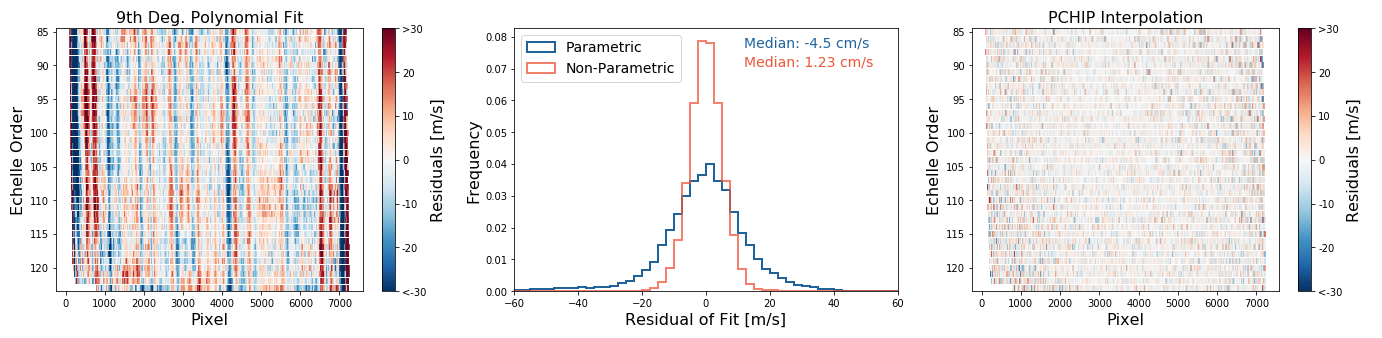
\includegraphics[width=\textwidth]{Figures/parametricTest.png}
%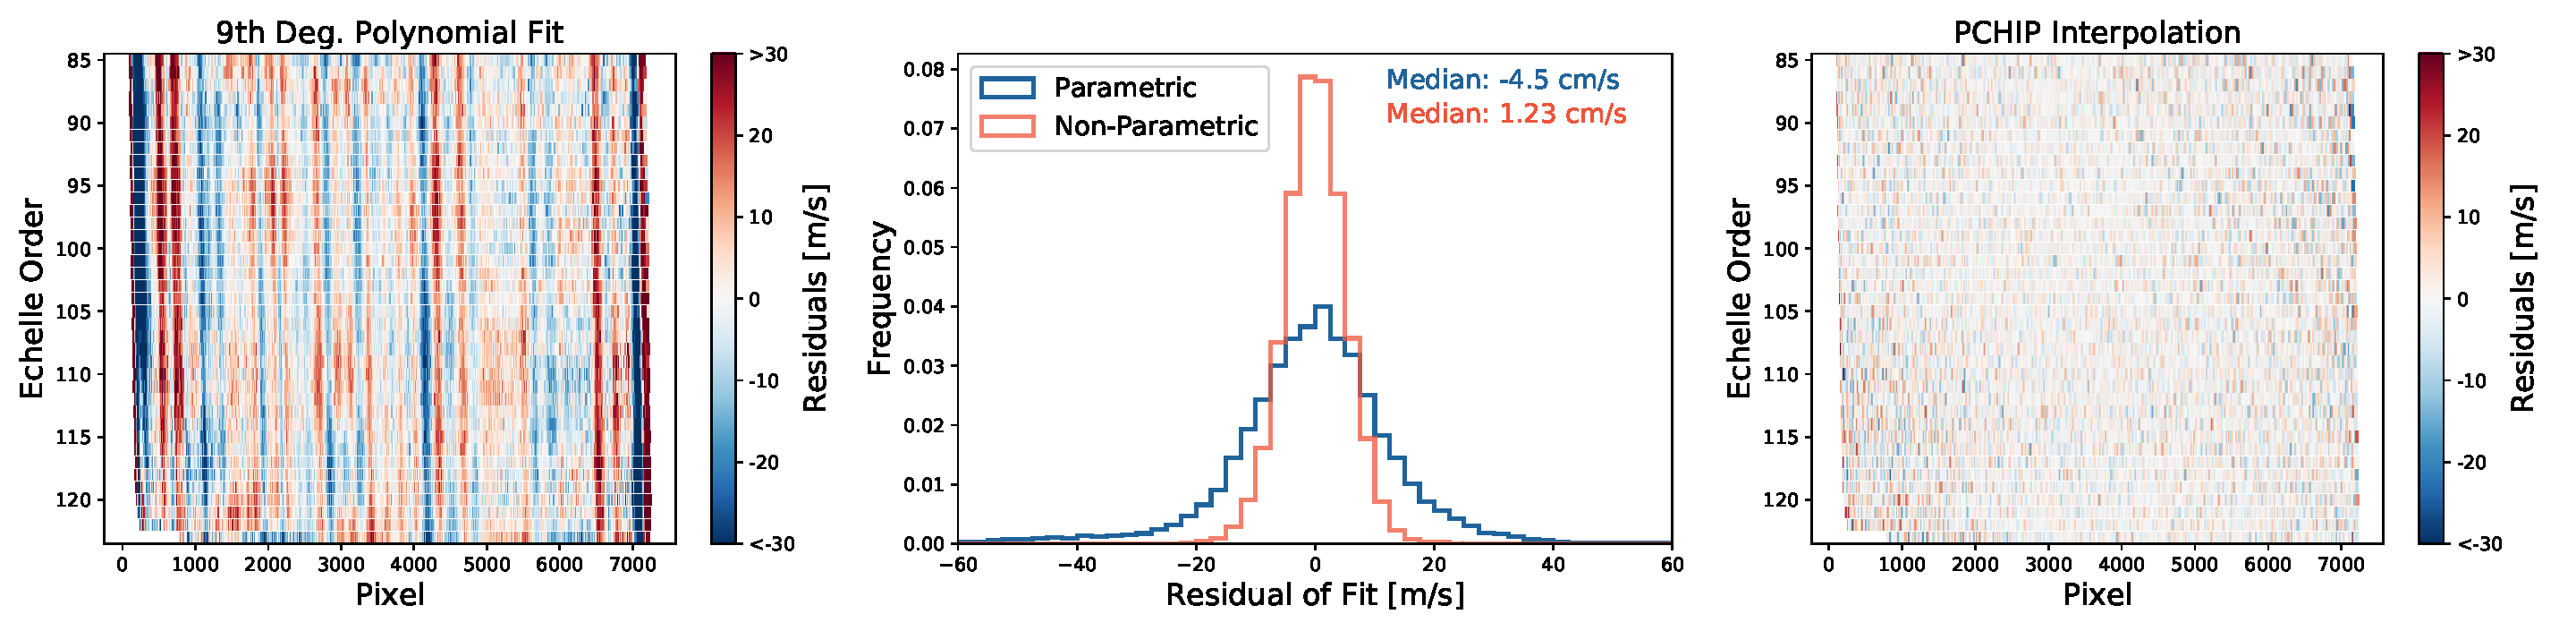
\includegraphics[width=\textwidth]{Figures/parametricTest.pdf}
\caption{Comparison of residuals to a parametric model (left-most) vs. a non-parametric model (right-most).  In each case, the color bar shows the difference between the predicted wavelength and the true wavelength for each line in units of velocity shift.  The center plot shows a histogram of the residuals of the polynomial fit (blue) and the non-parametric fit (green).  Medians of the residuals for each model are given in the top-right corner of the center plot in their corresponding colors.}
\label{fig:parametricTest}
\end{figure*}

We run the test using a polynomial derived as described in \lz{Petersburg2020} with discussed improvements.  We repeat the test using a PCHIP cubic-spline as a model rather than a polynomial.  The results are shown in Figure \ref{fig:parametricTest}.  For each method, we plot each line with respect to order and x-pixel and colored by the difference between the predicted and assigned wavelength for that line in units of $\mps$.

The residuals of the parametric model are shown in the left-most plot of Figure \ref{fig:parametricTest} while the residuals of the non-parametric model are shown in the right-most plot.  The center plot is a histogram of the residuals of the two methods.  The residuals from using the non-parametric model show less structure, are less spread around zero, and more symmetric about zero.  The non-parametric model was able to account for the high-order detector defects that are smoothed over by a polynomial fit, resulting in a more accurate fit.

\begin{figure*}[h]
\centering
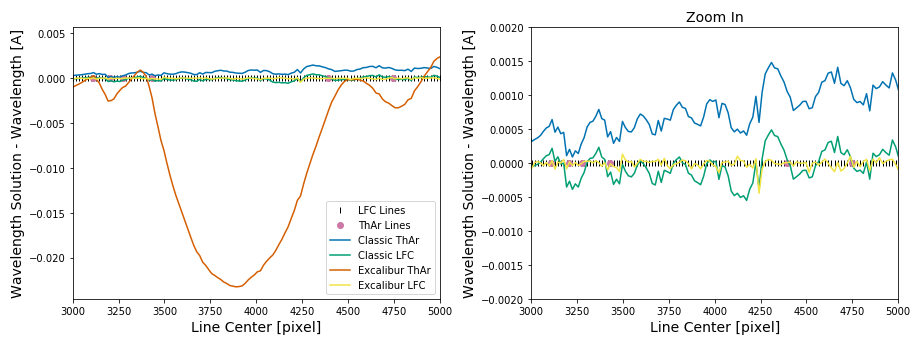
\includegraphics[width=\textwidth]{Figures/waveResids.png}
\caption{Comparisons of parametric and non-parametric wavelength solutions using either just ThAr lines or LFC lines. Left: the difference between each wavelength solution evaluated at the position of the LFC lines and the assigned wavelength of that LFC line.  The right plot is simply a zoom in of the left plot.  Note the large deviation when trying to implement Excalibur with just ThAr lines, which are much fewer in number.  The classic, polynomial  fit exhibits similar residuals regardless of whether the set of ThAr lines or LFC lines are used.  Excalibur using LFC lines exhibit the lowest residuals.}
\label{fig:waveResids}
\end{figure*} 

Incorporating a hierarchical, de-noising element results in ever better residuals!

\lz{come on, future Lily, add more here}

\begin{figure}[h]
\centering
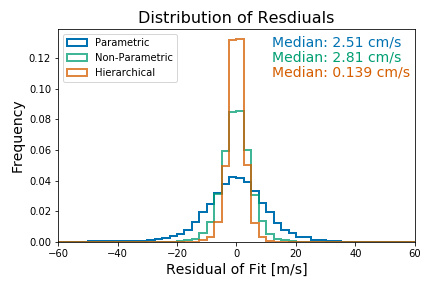
\includegraphics[width=0.5\textwidth]{Figures/allHists.png}
\caption{Histogram of residuals for different wavelength calibration methods.  The parametric (blue) and non-parametric (green) histograms are the same as described in Figure \ref{fig:parametricTest}.  In orange is the histogram of residuals to the full Excalibur model, which includes the hierarchical component.  The median of the residuals for each model is given in the top-right corner in each model's corresponding color.}
\label{fig:allHists}
\end{figure} 

\section{Real Data Through to RVs} \label{sec:realdata}
\lz{Debra and RP currently working through this.  Results seem good}

\section{Choice Choices} \label{sec:choices}
The implementation of  \name presented here required determining global variables and methods that we believe are or are close to optimal for constructing a high-fidelity wavelength solution.  This section will describe each choice and the associated decision-making process.

\subsection{Value of K}
The value of $K$ determines how many principal components are used to reconstruct the de-noised line centers.  This $K$ needs to be large enough so that all variability in the spectrograph is captured.  Too large, however, and the reconstruction will incorporate noise, thereby defeating the purpose.

We settled on a $K$ value of 6.  Figure \ref{fig:pcLfc} shows the first 6 principal components constructed using LFC lines.  In both cases there is clear structure in the first and second principal components.  The diagonal-banding structure seen in components 3, 5, and 6 we believe are capturing detector fabrication defects.  Components 3 and 4 show aberrant behavior on the edges of the two bluest orders, where lower signal results in more variation in the line fits.

\begin{figure*}[t]
\centering
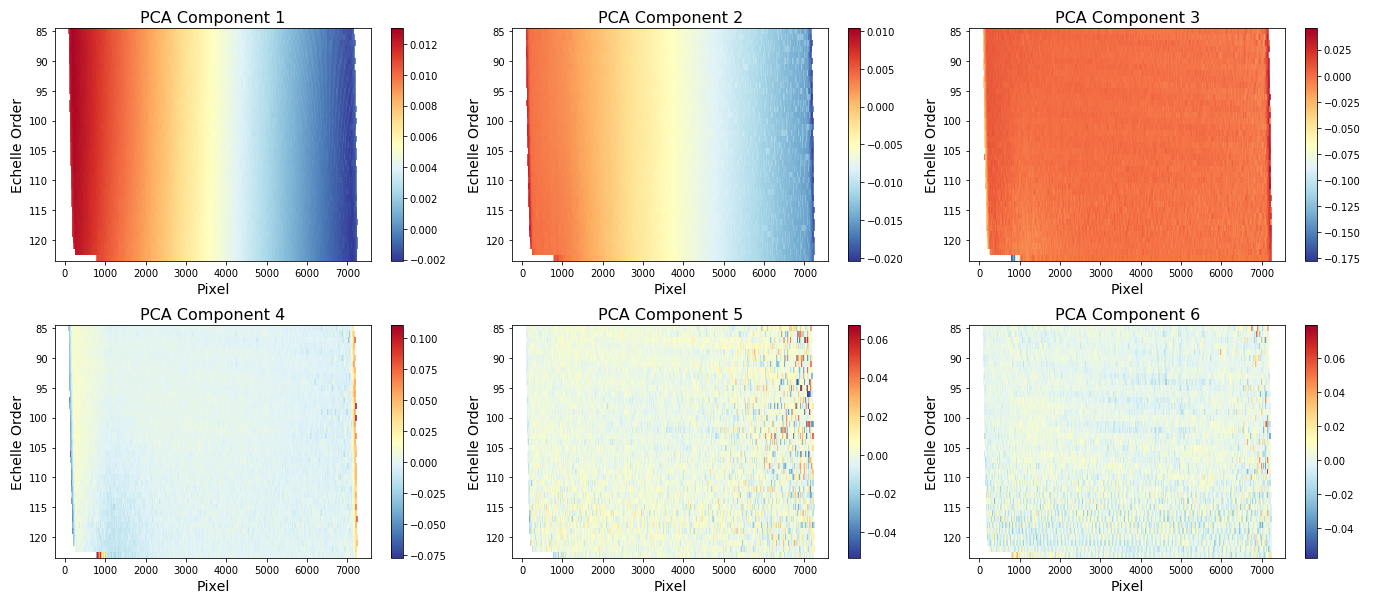
\includegraphics[width=\textwidth]{Figures/pcsLfc6.png}
%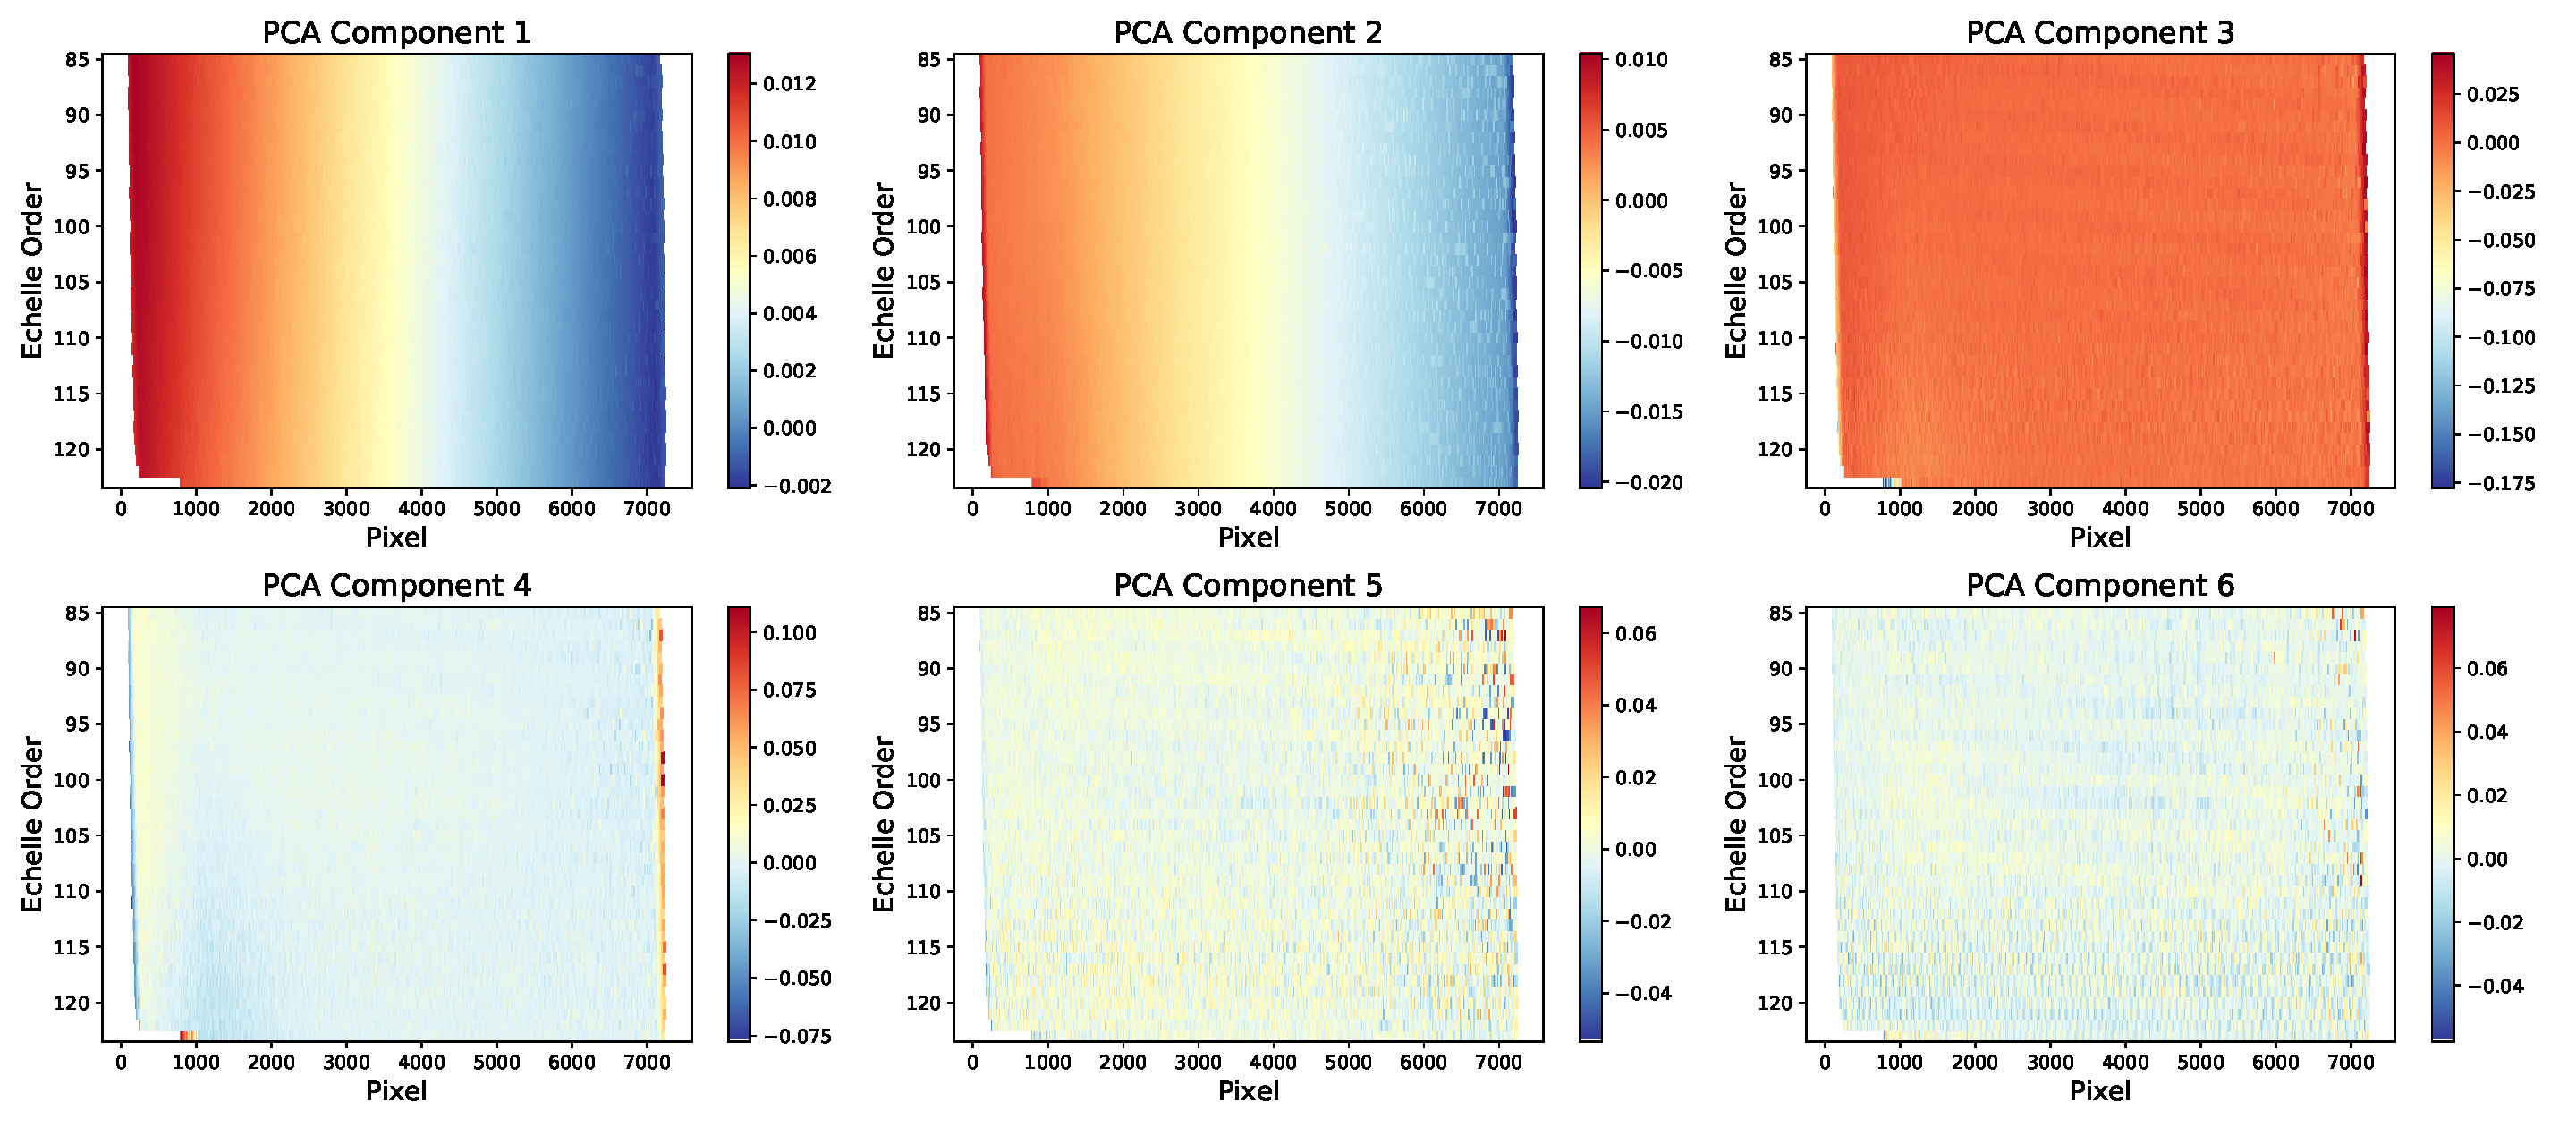
\includegraphics[width=\textwidth]{Figures/pcsLfc6.pdf}
\caption{The first six principal components constructed using only LFC lines.  There is clear structure for the first two principal components, though no order information is given to the PCA.  Principal components 3, 5 and 6 show some slight diagonal-banding structure, which we believe to be due to detector defects.  There is aberrant behavior in the bluest lines of the bluest two orders, which will be highlighted in the discussion.}
\label{fig:pcLfc}
\end{figure*}

In deciding a K value, we ran training-validation tests for K values spanning from 2 to 512.  One would expect the returned wavelengths to get increasingly more accurate with larger K until components that represent only noise are incorporated.  We found that the returned wavelengths are most accurate with a K value of 32.  However, the improvement is slight with K values greater than 6.  Comparisons of wavelengths returned by a K=6 model vs. a K=32 model show significant differences in less than 10, bluer lines.

\subsection{Interpolation of $a_{nk}$ with Respect to Time}
Figure \ref{fig:nightlyVariation} shows the amplitude of the first and second principal component with respect to time on the left.  Though the shape of the amplitudes with respect to time, a clear linear trend exists within each night.  This is shown by the right plots in Figure  \ref{fig:nightlyVariation}.  As the beginning-of-night and end-of-night calibration sets always include LFC exposures, we use a simple linear interpolation to interpolate principal component amplitudes with respect to time.

\lz{Yeah, the right-figure is kind of a mess, isn't it?}

\begin{figure*}[h!]
\centering
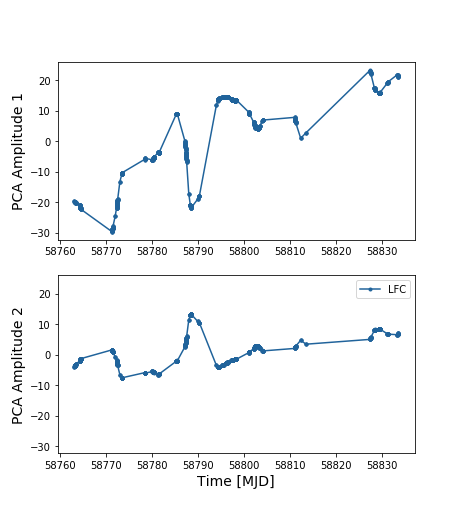
\includegraphics[width=0.56\textwidth]{Figures/pcA_lfc.png}
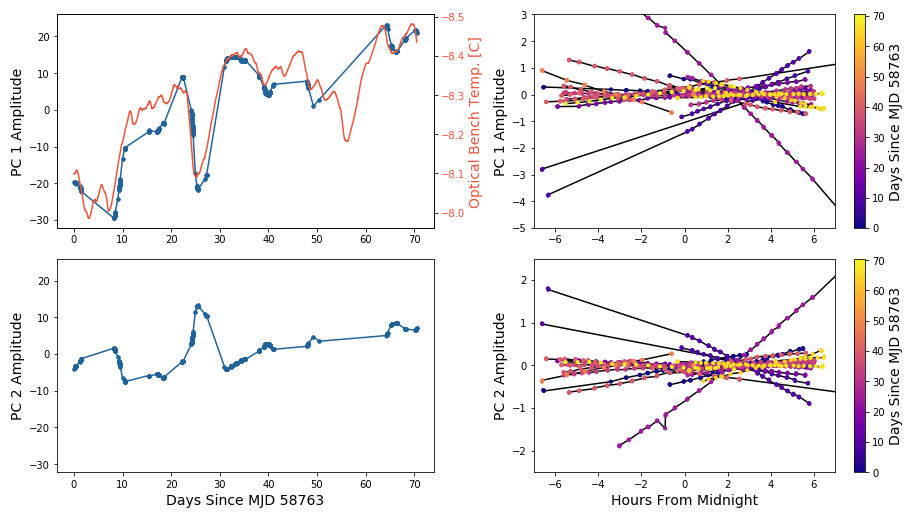
\includegraphics[width=0.42\textwidth]{Figures/pcAs_byDay.png}
\caption{Amplitude of the first two principal components show as a function of time (left) or fraction of a day (right).  Points mark the times at which we have calibration data.  Lines show the result of a linear interpolation.  Left: amplitudes as a function of time for both LFC (blue) and ThAr (green).  The top plot shows the amplitudes for the first principal component while the bottom plot shows the amplitudes for the second principal component.  The shape of the curves is similar regardless of calibration source.
Right: amplitudes of the first two principal components determined by the LFC exposures only.  Here, exposures are grouped by day and plotted with respect to what time of day the exposure was taken.  A linear interpolation through all the LFC exposures taken in one day are shown as black line.  Points are colored by the MJD of the exposure.  For each day, the amplitude has been artificially offset by the median amplitude for that day so all days are roughly on the same scale.}
\label{fig:nightlyVariation}
\end{figure*} 

\subsection{Interpolation of Wavelengths with Respect to Pixel}
Interpolation of wavelengths over pixel  is done order by order using a Piecewise Cubic Hermite Interpolating Polynomial (PCHIP) interpolator.  This interpolation incorporates the flexibility needed to model the changing dispersion of the spectrograph across an order along with any detector defects while also enforcing monotonicity.

Due to the dispersion intrinsic to echelle spectrographs, the wavelength change between pixels is greater at greater wavelengths.  This means that the function of wavelength vs. pixel across an order will always be monotonically increasing and concave down everywhere.  Consequently, linear interpolation of this function will systematically give erroneously low values.

A more classic cubic spline interpolation can run into issues with arc lines, which are irregularly spaced or even blended and so can appear very close together.  Very close lines cause huge deviations from the correct wavelengths, as seen in the green line of Figure \ref{fig:xinterp}..

\begin{figure*}[h]
\centering
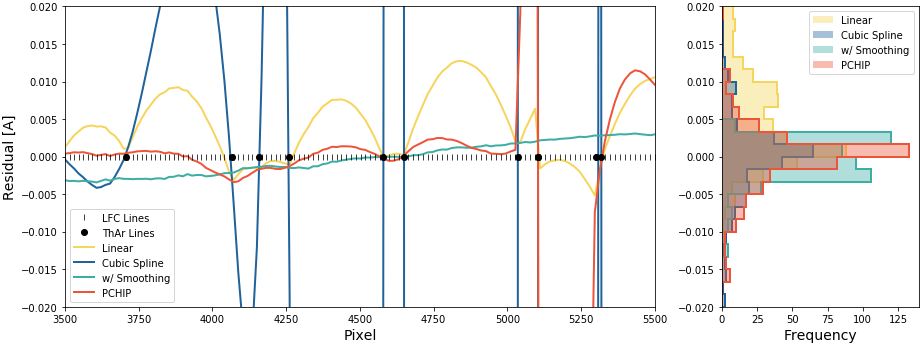
\includegraphics[width=\textwidth]{Figures/intpx_tests.png}
\caption{Results from different interpolation schemes over pixels.
Left: resultant wavelength solutions generated using ThAr lines, shown as green points.  Different interpolation schemes are shown in different colors.  The largest deviation comes with the classic cubic spline (green).
Right: histograms of residuals for each method when used to predict the wavelengths of LFC lines, shown as black, vertical lines.  The linear interpolation model (yellow) of this concave down relation is asymmetric with disproportionately positive residuals.  The popular cubic spline residuals (green) has very spread out residuals.  The residuals from an interpolation scheme that incorporates smoothing (blue) appear non-Gaussian with a plateau about zero.  Residuals from the PCHIP interpolator (orange) has the strongest peak at 0 and is roughly Gaussian.}
\label{fig:xinterp}
\end{figure*} 

These huge digressions can be avoided by allowing for some smoothing in the interpolation.  In Figure \ref{fig:xinterp}, we show an example in blue using scipy's Univarate Spline method.  While the result appears to follow the calibration lines much better, the smoothing ultimately causes larger residuals that are spatially correlated (Fig. \ref{fig:xinterp}, right).

For all orders, the edges will be overestimated while the middle will be underestimated.  This indicates that the smoothing is causing the resultant wavelength solution to underestimate the curvature of the pixel-wavelength relation, resulting in similar issues as with an inflexible, parametric model.  This enforces a smoothness we have no reason to believe is true for the data.

We instead turn to the PCHIP interpolator, which damps down huge deviations in the traditional cubic spline by requiring the resulting interpolated function to be monotonic.  This is a constraint we know is true from optics, since interpolation in the pixel direction is carried out order-by-order.  In Figure \ref{fig:xinterp} we show that using the PCHIP interpolator returns the lowest residuals.

\subsection{Order of Interpolation}
Why do we interpolate in time first and then in x?

\lz{We talked about including this discussion, but there is no real reason for doing things in this order except it is quite a bit faster.}


\section{Discussion} \label{sec:discussion}
\lz{I feel like we have a lot of hopes for this discussion section, which is not matched by my understanding of how to structure this discussion section.  For now, I have just written brief snippets that address each of the notes I have of things we have said we want to include.}

Generalization to etalon:
All methods described here are easily adapted to use with an etalon or any other arc lamp for which a list of lines and their assigned wavelengths can be constructed.

Ability to vet for bad exposures:
An advantage of using PCA on all LFC exposures and line positions is the ability to isolate exposures that exhibit unexpectedly large variation.  Such variation is likely to be captured by an early principal component.  Errant exposures will be singled out by a spike in the amplitude for just that principal component.  This allowed us to quickly find flawed LFC exposures, which otherwise would have required visual inspection of all 1200+ LFC exposures.

Changes in instrument/change point detection:
On the other hand, this same feature of using PCA can also be seen as a bug.  PCA is good at picking up on variation regardless of the source of the variation.  Any variation that breaks our assumption of an instrument that exists in only a low-dimensional calibration space will likely be captured by early principal components, which will no longer serve to denoise the calibration data.  We found that violations of this stability assumption typically manifests as change points in the principal component amplitudes with respect to time.

Sensitivity to line-position fitting:
The PCA will also be sensitive to variations in line fitting.  For example, if certain regions have lines of lower signal, variable background, or are otherwise harder to fit, any resultant variation in the returned line positions across different exposures will also be captured by any PCA.  High-fidelity line positions are essential to ensure the PCA is capturing variations in the spectrograph's calibration rather than changes in how well a line can be fit.

Perfect degeneracy problem:
With any wavelength solution, there is a perfect degeneracy between what is defined as the ``center of the line'' and the resultant wavelength solution.  If, for example, a cross correlation method is used to extract RVs from the data, a systematic difference may be introduced depending on the definition of the center of the line.  In principle, the best way to mitigate this error would be to use a calibration source that looks like a star.

Self calibration idea:
Once we define a calibration space that captures all possible degrees of freedom for a stabilized spectrograph, then all exposures taken with the spectrograph contain information about where the spectrograph lies in that space at the time of the exposure.  Meaning, a science exposure can be used to determine the current state of the instrument in this calibration space.  It would therefore be possible to self-calibrate science exposures without the use of an additional wavelength calibration source.

How hard would it be to go bayesian?  Description of other implementations of \name\ than what we did here?

\end{document}
